%\subsubsection{Desenvolvimento}

	%01 - Criação do database
	
	\par Com o ambiente de desenvolvimento pronto, começou de fato o
desenvolvimento. Primeiramente foi necessário criar o banco de dados no SGDB.
Este por sua vez foi criado com a ajuda do PgAdmin que é um software gráfico
para administração do SGDB, e que fornece uma interface gráfica de apoio para o
PotgreSql. Para criar era necessário ja estar com o PgAdmin aberto e conectado
a um servidor de banco de dados que neste caso era em servidor local como pode
ser visto na Figura \ref{fig:desws}.

	\begin{figure}[h!]
		\centerline{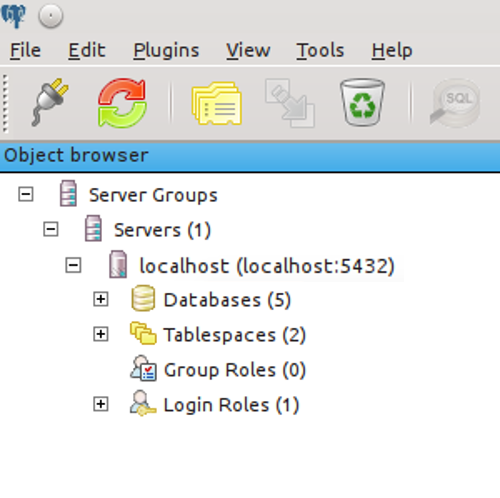
\includegraphics[scale=1]{./imagens/2_q_metodologico/4_procedimentos_resultados/43_webservice/432_desenvolvimento/desws.png}}
		\caption[Servidor de banco de dados local no PgAdmin]{Servidor de banco de
		dados local no PgAdmin.
			\textbf{Fonte:}Elaborado pelos autores.}
		\label{fig:desws}
	\end{figure}
	
	\pagebreak
	
	\par Para a efetiva criação do banco de dados era necessário clicar com o
botão direito do \textit{mouse}, sobre a opção \textbf{Databases -> New
Database\ldots} no PgAdmin, apresentada na Figura \ref{fig:desws1}.

	\begin{figure}[h!]
		\centerline{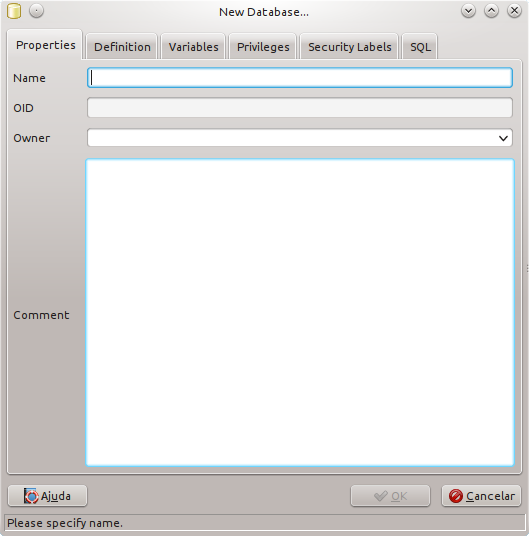
\includegraphics[scale=0.8]{./imagens/2_q_metodologico/4_procedimentos_resultados/43_webservice/432_desenvolvimento/desws1.png}}
		\caption[Opção \textit{New Database\ldots}]{Opção \textit{New Database\ldots}.
			\textbf{Fonte:}Elaborado pelos autores.}
		\label{fig:desws1}
	\end{figure}

	\pagebreak
	
	\par Em seguida foi necessário preencher o dados da janela apresentada, como
está apresentado na Figura \ref{fig:desws2}.
	
	\begin{figure}[h!]
		\centerline{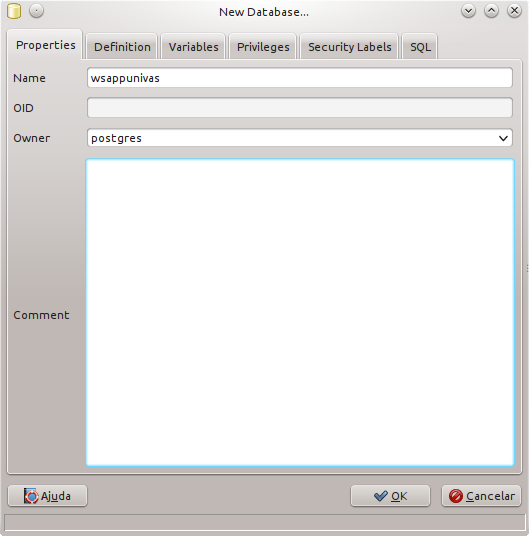
\includegraphics[scale=1]{./imagens/2_q_metodologico/4_procedimentos_resultados/43_webservice/432_desenvolvimento/desws2.png}}
		\caption[Tela \textit{New Database\ldots}]{Tela \textit{New Database\ldots}.
			\textbf{Fonte:}Elaborado pelos autores.}
		\label{fig:desws2}
	\end{figure}
	
	\pagebreak

	\par Como pode ser visto foram preenchidos os campos nome e usuário . O campo
nome se refere ao nome do banco de dados que foi definido com
\texttt{wsappunivas}, e usuário, o responsável pelo banco de dados, que para
este caso foi usuário padrão do SGDB, que é o \texttt{postgres}. Além destas
configurações mais nenhuma foi necessária. O banco de dados foi criado, porém
sua estrutura não foi definida, pois como será visto mais adiante o Hibernate,
possui um mecanismo, que com algumas configurações, permite a estruturação do
banco de dados, de acordo com o mapeamento objeto-relacional. Isto permitirá
mudanças na estrutura do banco de dados e suas tabelas, e até mesmo eventuais
correções.
	
	%02 - Início do projeto web no eclipse;
	\par Em seguida foi criado um projeto do tipo Dynamic Web Project no
Eclipse. Para proceder com a criação de um novo projeto deste tipo no Eclipse, é
necessário acessar na IDE, a opção \textbf{File -> New-> Dynamic Web Project}
como pode ser visto na figura \ref{fig:desws3}.

	
	\begin{figure}[h!]
		\centerline{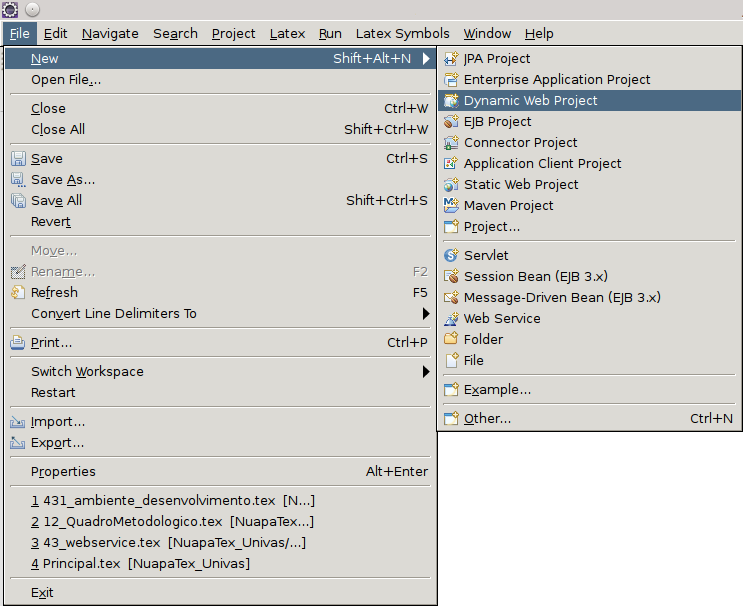
\includegraphics[scale=0.8]{./imagens/2_q_metodologico/4_procedimentos_resultados/43_webservice/432_desenvolvimento/desws3.png}}
		\caption[Tela \textit{New Database\ldots}]{Tela \textit{New Database\ldots}.
			\textbf{Fonte:}Elaborado pelos autores.}
		\label{fig:desws3}
	\end{figure}
	
	\pagebreak
	
 	\par Em seguida foi apresentada uma tela para o preenchimento de alguns dados
 requeridos para a criação do projeto. Destas informações somente foi preenchido
 o nome do projeto. As outras informações continuaram sendo as que vem por
 padrão da IDE. A janela apresentada e as informações preenchidas podem ser
 vistas na Figura \ref{fig:desws4}.

	\begin{figure}[h!]
		\centerline{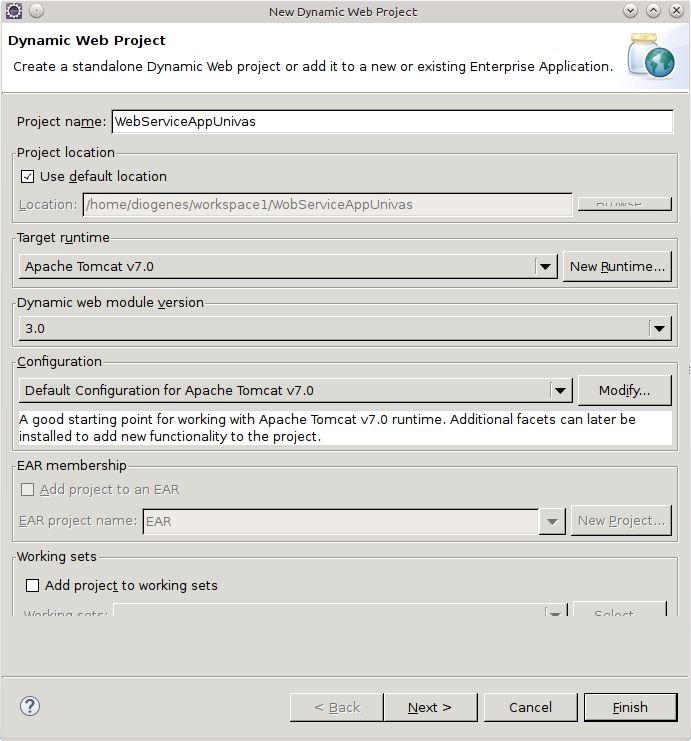
\includegraphics[scale=0.8]{./imagens/2_q_metodologico/4_procedimentos_resultados/43_webservice/432_desenvolvimento/desws4.png}}
		\caption[Tela para criação de um novo projeto no Eclipse]{Tela para criação de um novo projeto no Eclipse.
			\textbf{Fonte:}Elaborado pelos autores.}
		\label{fig:desws4}
	\end{figure}
	
	\pagebreak
	
	
	\par Na próxima janela apresentada, que têm por função configurar a pasta de
códigos do projeto manteve-se a configuração apresentada pela IDE, como mostra
a Figura \ref{fig:desws5}.

	\begin{figure}[h!]
		\centerline{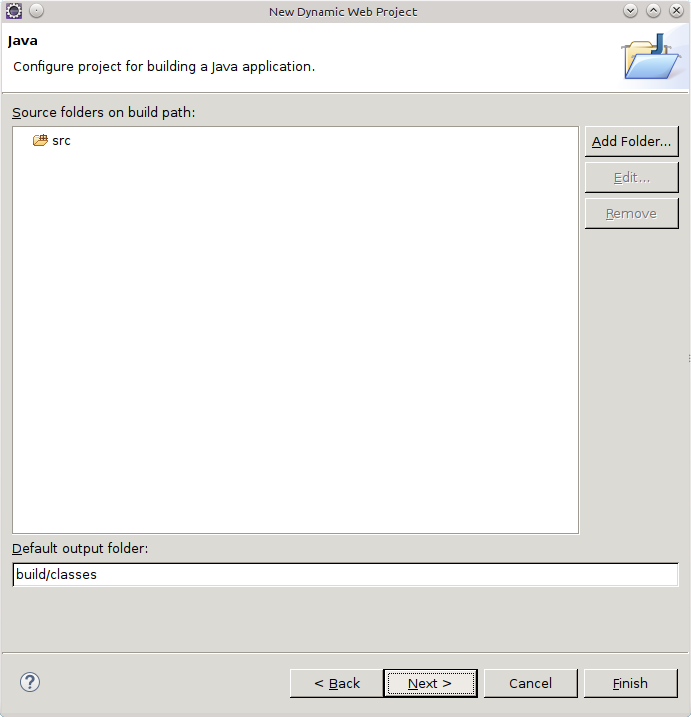
\includegraphics[scale=0.8]{./imagens/2_q_metodologico/4_procedimentos_resultados/43_webservice/432_desenvolvimento/desws5.png}}
		\caption[Tela para criação de um novo projeto no Eclipse]{Tela para criação de um novo projeto no Eclipse.
			\textbf{Fonte:}Elaborado pelos autores.}
		\label{fig:desws5}
	\end{figure}
	
	\pagebreak
	
	\par Na sequencia, na tela que foi apresentada era necessário cadastrar
preencher o campo \textbf{Context root:} com o contexto principal da aplicação
web que acabou mantendo o próprio nome da aplicação. Além disso foi marcado a
opção \textbf{Generate web.xml deployment descriptor}, para que ao criar o
projeto, a própria IDE criasse o arquivo \texttt{web.xml}, arquivo responsável
por algumas configurações da aplicação web. Esta tela esta apresentada na
Figura \ref{fig:desws6}.

	\begin{figure}[h!]
		\centerline{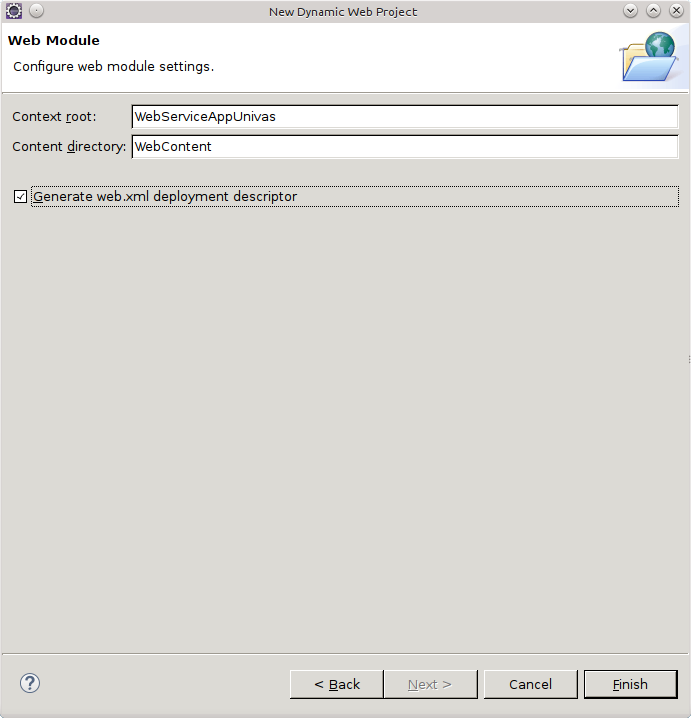
\includegraphics[scale=0.8]{./imagens/2_q_metodologico/4_procedimentos_resultados/43_webservice/432_desenvolvimento/desws6.png}}
		\caption[Tela para criação de um novo projeto no Eclipse]{Tela para criação de um novo projeto no Eclipse.
			\textbf{Fonte:}Elaborado pelos autores.}
		\label{fig:desws6}
	\end{figure}
	
	\pagebreak

	%03 - Mapeamento orm;	
		%	->Criação do pacote

	\par Após este passo foi concluído a criação do projeto, e já era possível
iniciar os trabalhos com a camada de persistência de dados do projeto. Para
este propósito, primeiramente foi criado um pacote, onde ficaram contidas as
classes que representam as entidades do ORM. Para a criação do pacote foi
necessário clicar com o botão direito do mouse sobre o projeto e acessar a opção
\textbf{New -> Package}, como pode ser visto na Figura \ref{fig:desws7}.

	\begin{figure}[h!]
		\centerline{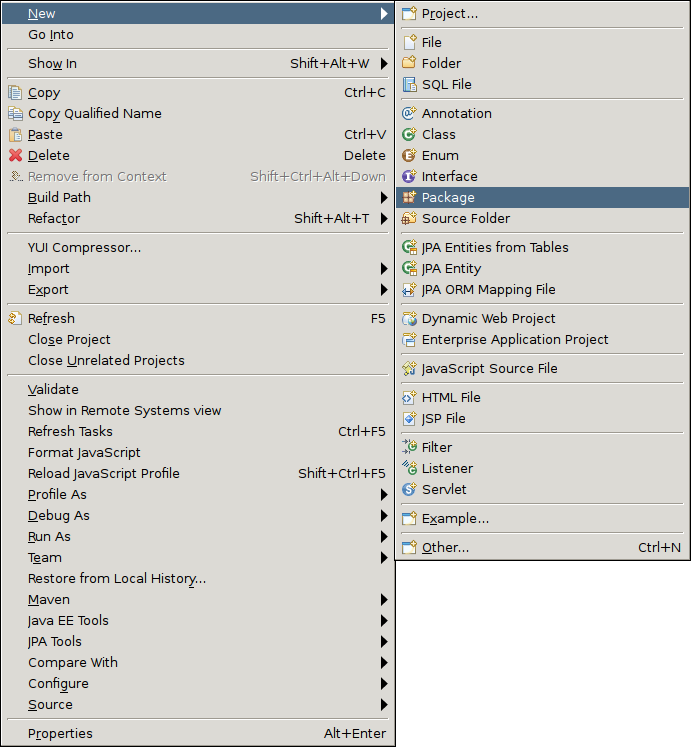
\includegraphics[scale=0.8]{./imagens/2_q_metodologico/4_procedimentos_resultados/43_webservice/432_desenvolvimento/desws7.png}}
		\caption[Tela para criação de um novo projeto no Eclipse]{Tela para criação de um novo projeto no Eclipse.
			\textbf{Fonte:}Elaborado pelos autores.}
		\label{fig:desws7}
	\end{figure}
	
	\pagebreak 
	
	\par Em seguida foi apresentado a tela para a criação de um novo pacote
mostrada na Figura \ref{fig:desws8}. O pacote recebeu o nome de
"\texttt{br.edu.univas.restapiappunivas.model}", pois nele estão contidas as
classes que fazem parte do modelo de negócios da aplicação. Este pacote foi
criado visando a divisão das responsabilidades internas no projeto, além de
contribuir positivamente com a organização do mesmo.

	\begin{figure}[h!]
		\centerline{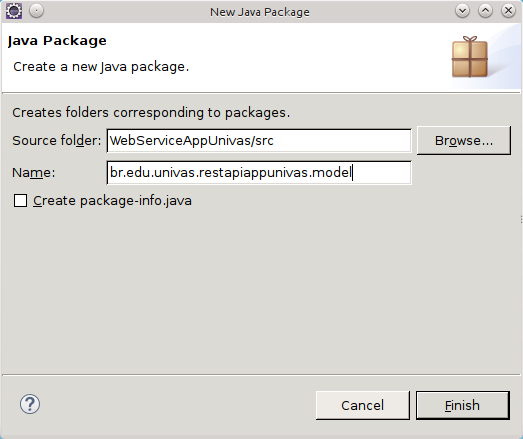
\includegraphics[scale=0.8]{./imagens/2_q_metodologico/4_procedimentos_resultados/43_webservice/432_desenvolvimento/desws8.png}}
		\caption[Tela para criação de um novo projeto no Eclipse]{Tela para criação de um novo projeto no Eclipse.
			\textbf{Fonte:}Elaborado pelos autores.}
		\label{fig:desws8}
	\end{figure}
	
	\pagebreak


		
		%	->Criação das classes
	\par Com este pacote criado, ja era possível criar as classes do ORM. Foi
criada primeiramente a classe \texttt{Student.java}. Para que esta classe
pudesse ser reconhecida como um entidade e persistida ao banco de dados através
do Hibernate, é necessário que esta classe tivesse a anotação
\texttt{@Entity}. Com isso esta classe ja poderia ser entendida como uma
entidade e poderia ser persistida no banco de dados, porém além dessa anotação
outras foram usadas para que a persistência pudesse ocorrer de forma
consistente.





	
	
			
	
		\par Fazendo uso desse diagrama foi possível criar todas as classes 
	Java que representam as entidades do mapeamento objeto-relacional. 
	Essas classes foram criadas fazendo uso de anotações próprias do
	Hibernate, que é um \textit{framework} que implementa a especificação
	JPA\footnote{JPA - Java Persistense API}. Essas classes fazem parte
	dos mecanismos de persistêcia de dados e são simplesmente t ou seja, objetos
	simples que contêm somente atributos privados e os métodos \textit{getters} e
	\textit{setters} que servem apenas para encapsular estes atributos. Uma das
	classes criadas, foi a classe \texttt{Aluno.java} que representa a tabela
	\texttt{alunos} no banco de dados e está representada.
		
		\par Foram criadas outras classes Java com a mesma finalidade da
	anterior, porém com pequenas diferenças no que diz respeito à atributos,
	metodos e anotações. Estas classes representam, de maneira individual, as
	tabelas no banco de dados. Certos atributos dessas classes têm por finalidade
	representar as colunas de cada tabela. Já os atributos que armazenam instâncias
	de outras classes ou até mesmo conjuntos (coleções) de instâncias representam os
	relacionamentos entre as tabelas. 
	
		%04 - HashCode e equals
		\par E por fim, para cada classe querepresenta uma 	entidade, foi necessário
	implementar os métodos \texttt{hashCode} e \texttt{equals}, para que estas
	pudessem facilmente ser comparadas e diferenciadas em relação aos seus
	valores, haja visto que cada instância destas classes representa um registro
	no banco de dados.
		
		%05 - Configuração do persistence.xml
		\par Em seguida à criação das entidades, foi necessário configurar o arquivo
	\texttt{persistence.xml} que fica dentro do \textit{classpath} do projeto
	Java ou seja, dentro da mesma pasta onde estão contidos pacotes do
	projeto. Este arquivo é extremamente importante, pois é nele que estão todas
	as configurações relativas à conexão com o banco de dados, configurações
	referentes ao Dialeto SQL que vai ser usado para as consultas e configurações
	referentes ao \textit{persistence unit} que é o conjunto de classes mapeadas
	para o banco de dados.	O arquivo \texttt{persistence.xml} está exposto no
	código \ref{fig:qm11}.
	
 		\begin{figure}[h!]
			\centerline{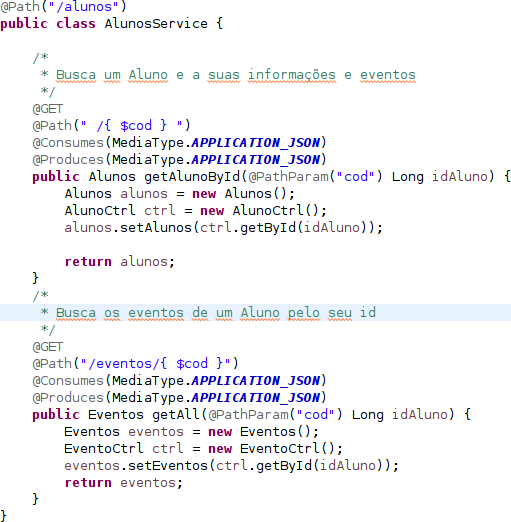
\includegraphics[scale=0.6]{./imagens/2_q_metodologico/qm11.png}}
			\caption[Arquivo \texttt{persistence.xml}]{Arquivo \texttt{persistence.xml}.
			\textbf{Fonte:}Elaborado pelos autores.}
			\label{fig:qm11}
		\end{figure}
		
			%06 - Confecção JpaUtil.java
			\par Em seguida à confecção do \texttt{persistence.xml} foi criada a
		classe \texttt{JpaUtil} que está representada na Figura \ref{fig:qm12}.
		Esta classe é responsável por criar uma \texttt{EntityManagerFactory} que é
		uma  fábrica de instâncias de \texttt{EntityManager} que nada mais é que um
		\textit{persistence unit} ou unidade de persistência. Essa classe tem a
		responsabilidade de prover um modo de comunicação entre a aplicação e o banco
		de dados. No entanto a classe \texttt{JpaUtil} cria uma única instância de
		\texttt{EntityManagerFactory}, que é responsável por disponibilizar e
		gerenciar as instâncias de \texttt{EntityManager} de acordo com a necessidade
		da aplicação.
		
		\pagebreak
		\begin{figure}[h!]
			\centerline{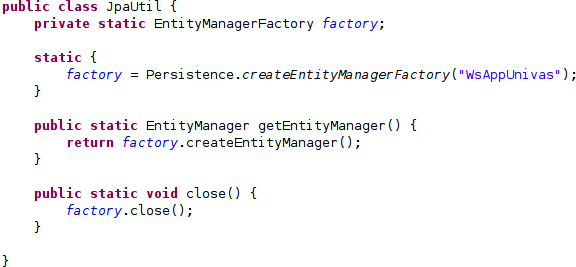
\includegraphics[scale=0.7]{./imagens/2_q_metodologico/qm12.png}}
			\caption[Classe \texttt{JpaUtil}]{Classe \texttt{JpaUtil}.
			\textbf{Fonte:}Elaborado pelos autores.}
			\label{fig:qm12}
		\end{figure}
		
	\par Em seguida à construção das classes que fazem a parte da persistência de
dados, foi desenvolvido a parte de disponibilização de serviços
RESTful, fazendo uso do \textit{framework} Jersey. Com isso
pode-se construir a classe que representa o primeiro serviço do
\textit{webservice}, que é a classe \texttt{Alunos}. Essa classe representa um
contexto REST, e portanto, dispõe de alguns recursos. Esses recursos fazem a
recuperação e a transmissão dos dados do \textit{web service} para o aplicativo
Android. Essa classe e seus respectivos métodos  estão representada na
Figura \ref{fig:qm13}.

		\begin{figure}[h!]
			\centerline{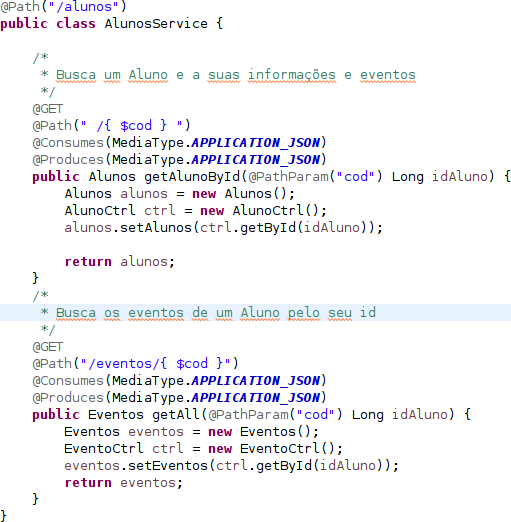
\includegraphics[scale=0.7]{./imagens/2_q_metodologico/qm13.png}}
			\caption[Classe \texttt{AlunosService}]{Classe \texttt{AlunosService}.
			\textbf{Fonte:}Elaborado pelos autores.}
			\label{fig:qm13}
		\end{figure}
		
		\par O \textit{webservice} pode fazer a busca de alunos pelo \texttt{id}
passado ou retornar uma coleção de eventos vinculados a um alunos, dependendo
do recurso acessado. Os tipos de dados que o \textit{webservice} consome e
retorna é o JSON\footnote{JSON - Javascript Object Notation}. Não foi
necessário fazer nenhuma implementação adicional relativa a este formato, pois
o próprio \textit{framework} Jersey faz o tratamento e a conversão dos tipos de
entrada e saída de dados. No caso do saída de dados, faz a conversão de objetos 
Java para JSON. E no caso de entrada tranforma um JSON em objeto
Java já conhecido pelo \textit{web service}. Com isso concluiu-se o
desenvolvimento do \textit{web service} que fornece os dados para o aplicativo.

	%23 - Módulo que ira fazer a busca dos dados na base da instituição de ensino
	%24 - Falar que vai ser simulado
	\par Para que fosse possível transmitir dados para o aplicativo, era
necessário receber as informações do sistema acadêmico da referida instituição,
haja vista que o \textit{web service} é independente do mesmo. Para esse
propósito é necessário  contruir um módulo que faça a importação dos dados
necessários para a base de dados do \textit{web service}. 

	\par Este por sua vez terá a responsabilidade de fazer a importação dos dados
periodicamente, e ainda tratar os tipos de dados recebidos para tipos
aplicáveis ao banco de dados local. Além disso é preciso notificar o módulo
responsável por invocar o serviço Google Cloud Messaging para que os
dispositivos dos alunos aos quais houveram atualizações nos dados, fossem
notificados e fizessem acesso ao \textit{web service} para solicitar esses
dados atualizados.

	\par Os procedimentos acima citados foram os passos até agora realizados com o
propósito de se alcançar os resultados esperados para essa pesquisa.



%pom.xml
\par Com a ajuda do plugin Maven. Esse Projeto foi criado usando o
Maven pois depende de uma quantidade considerável de \textit{frameworks}, e uma das
principais funcionalidades deste plugin, é ajudar na resolução das dependências
de um projeto Java.

	\par Para tal projeto foi necessário a configuração do \texttt{POM.xml} que é o
arquivo utilizado pelo Maven. Nele estão contidas as configurações
relativas à compilação do projeto bem como suas dependências.  Na figura
 a seguir pode ser visto o conteúdo do arquivo
\texttt{POM.xml}.






%07 - Explicar anotações dos pojos
%08 - Finalizando camada de persistência
%09 - Camada de serviço
%10 - Classes que disponibilizam serviços anotações
%11 - Explicar as entities criadas para disponibilizar os dados
%12 - Ctrls que fazem a busca dos dados
%13 - Problema do erro 500
%14 - Provedor de arquivos e contexto
%15 - Em todos citar o pom.xml
%16 - Configuração do web.xml
%17 - Módulo de varredura de atualizações com timerTask
%18 - Módulo de alerta de provas agendas no dia da prova
%19 - Configuração da conta no gcm
%20 - Módulo para disparar as mensagens para o gcm
%21 - Mostrar a estrutura do empacotamento depois de finalizado
%22 - Serviço que faz o registro de sender_id